\subsection{箭图的定义}

定义 1. —— 箭图是一个四元组 (S, F, o, t)，其中 S 与 F 是集合，o、t 是从 F 到 S 的映射。

设 \(C = (S, F, o, t)\) 为箭图。S 的元素称为 C 的顶点。F 的元素称为 C 的箭。设 f 为 C 的箭；顶点 \(o(f)\) 称为 f 的起点或源，顶点 \(t(f)\) 称为 f 的终点或靶；也说 f 连接顶点 \(o(f)\) 与顶点 \(t(f)\) 。映射 o 与 t 分别称为箭图 C 的源映射与靶映射，或起点与终点映射。

当 C 为箭图时，\(\operatorname{Som}(\mathrm{C})\) 、\(\operatorname{Fl}(\mathrm{C})\) 、\(o_{C}\) 与 \(t_{C}\) 分别表示 C 的顶点集、箭集、源映射与靶映射。设 a 与 b 为 C 的顶点；C 中连接 a 与 b 的箭所成的集记作 \(\operatorname{Fl}_{a,b}(\mathrm{C})\) ，或等价地记作 \(C_{a,b}\) 。

为便于理解推理，可以用由点与带箭头的线组成的图形来表示箭图，它们分别对应于顶点与箭。这个图形：

\pandocbounded{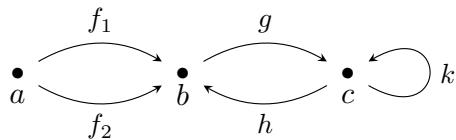
\includegraphics[keepaspectratio]{images/part001_552ae758.jpg}}

表示一个箭图，其顶点为 a、b、c，其箭为 \(f_{1}, f_{2}, g, h, k\) ，且源映射与靶映射由下式给出

\[
\begin{array}{c c c c} o (f _ {1}) = o (f _ {2}) = a & \quad o (g) = b & \quad o (h) = c & \quad o (k) = c \\ t (f _ {1}) = t (f _ {2}) = b & \quad t (g) = c & \quad t (h) = b & \quad t (k) = c. \end{array}
\]

